\documentclass{memoir}

\title{Linear Algebra: Design and Implementation}
\author{Rick Cui}
\date{01/22/2009}

\usepackage{graphicx, amsfonts, amssymb, amsmath, amsthm}
% This is for java code format.
\usepackage{listings}
% for bib
\usepackage[sectionbib]{natbib}
\usepackage{chapterbib}

% chapter header style
\usepackage{color,calc,soul,fourier}
\definecolor{nicered}{rgb}{.647,.129,.149}
\makeatletter
\newlength\dlf@normtxtw
\setlength\dlf@normtxtw{\textwidth}
\def\myhelvetfont{\def\sfdefault{mdput}}
\newsavebox{\feline@chapter}
\newcommand\feline@chapter@marker[1][4cm]{%
	\sbox\feline@chapter{%
		\resizebox{!}{#1}{\fboxsep=1pt%
			\colorbox{nicered}{\color{white}\bfseries\sffamily\thechapter}%
	}}%
\rotatebox{90}{%
	\resizebox{%
		\heightof{\usebox{\feline@chapter}}+\depthof{\usebox{\feline@chapter}}}%
	{!}{\scshape\so\@chapapp}}\quad%
	\raisebox{\depthof{\usebox{\feline@chapter}}}{\usebox{\feline@chapter}}%
}
\newcommand\feline@chm[1][4cm]{%
	\sbox\feline@chapter{\feline@chapter@marker[#1]}%
	\makebox[0pt][l]{% aka \rlap
	\makebox[1cm][r]{\usebox\feline@chapter}%
}}
\makechapterstyle{daleif1}{
	\renewcommand\chapnamefont{\normalfont\Large\scshape\raggedleft\so}
	\renewcommand\chaptitlefont{\normalfont\huge\bfseries\scshape\color{nicered}}
	\renewcommand\chapternamenum{}
	\renewcommand\printchaptername{}
	\renewcommand\printchapternum{\null\hfill\feline@chm[2.5cm]\par}
	\renewcommand\afterchapternum{\par\vskip\midchapskip}
	\renewcommand\printchaptertitle[1]{\chaptitlefont\raggedleft ##1\par}
}
\makeatother
\chapterstyle{daleif1}

% chapter mini toc
\usepackage{minitoc}

\newtheorem{thm}{Theorem}[section]
\newtheorem{cor}[thm]{Corollary}
\newtheorem{lem}[thm]{Lemma}

%============================================================================
\begin{document}
\DeclareGraphicsExtensions{.pdf, .png, .eps}
\setsecnumdepth{subsection}
%\settocdepth{subsection}
\maxsecnumdepth{subsection}



%\maketitle
%\pagebreak

% This is the front cover, TitleGM style
\begin{center}
\thispagestyle{empty}
\begingroup
	%\vspace*{\baselineskip} 
	\vfill 
	\hbox{% 
		\hspace*{0.03\textwidth}% 
		\rule{1pt}{\textheight} 
		\hspace*{0.05\textwidth}% 
		\parbox[b]{0.9\textwidth}{ 
			\vbox{% 
				\vspace{0.1\textheight} 
				{\noindent\HUGE\bfseries Numerical Linear Algebra :\\[0.5\baselineskip] 
					Design and Implementation}\\[2\baselineskip] 
				{\Large\itshape An Object-oriented Approach}\\[4\baselineskip] 
				{\Large Rick Cui}\par 
				\vspace{0.5\textheight} 
				{\noindent Wonderful World}\\[\baselineskip] 
			}% end of vbox 
		}% end of parbox 
	}% end of hbox 
	\vfill 
	\null 
\endgroup
\end{center}

\frontmatter

\dominitoc

\begin{center}

%put \addtocontents{toc}{\protect\thispagestyle{empty}}

%\thispagestyle{empty}
\setcounter{page}{1}
\tableofcontents
\end{center}

\incrementmtc

\pagestyle{headings}
\mainmatter
%\input{ack/ack.tex}
%\pagebreak

%********** Chapter 1 **********
\chapter{Matrix Design}
\minitoc

TO DO LIST

amsfont are better.

java code needs a better format: font and layout position.


There are already various packages available in Java for linear algebra, but most of them are dedicated to algorithms, such as solving linear equation systems. The main purpose of this package is to design matrices and their related behaviors at the proper abstract level from a software engineering point of view. Mathematical programming is harder than general software programming because of the heavy optimization embedded in the code. Designing matrix related classes are among the worst because matrix computing involves both performance and memory management. However, in the same spirit in mathematics where we always divide bigger problems into smaller problems, we hope we achieve a better design by utilizing some software design principles without sacrificing performance. Our goal is to design a reusable, flexible and easy to extend and test package.

\section{Scope}
This package has the following scope:
\begin{itemize}
\item All matrices are two dimensional.
\item All matrix cells are of type double.
\item Banded/Block matrices are not implemented.
\item Any parallel or divide-and-conquer based algorithms are not in the scope.
\end{itemize}
There are several reasons we limit ourselves to this scope:
\begin{itemize}
\item Though Java has a root class, Number, for all numeric classes, it's not operable arithmetically, such as $a + b$ where $a$ and $b$ are of type Number. Therefore, even we can extend Number class to Rational, Complex, or Quaternion, we really can't operate on them. The consequence is that we can't define a generic matrix interface which has getCell() and setCell() methods depending on Number class. If we have to extend Number, we would have to extend arithmetic operations through interfaces, such as addition and subtraction. This would make the code hard to read and maintain. 
\item The Java array is continuous in the memory. But arrays of array is not. This has a big performance hit, even in multiplications of matrices of type double. If we have array of arrays of Objects, the performance is getting worse.
\item Java doesn't support operator overloading and so even if we extend from the Number class to a Complex, we can't utilize the same code for doubles on Complex, such as arithmetic operations. Furthermore, we can't overload matrix operations either, otherwise we could easily extend the cell-based matrices to block-based matrices.
\item One way to expand to higher dimensional matrices, such as double[][][], one way is to define a new class to encapsulate the index various, e.g., a MatrixIndex class, then map the objects of this class to the matrix data storage. But we need to create a lot of objects of this class, one for each matrix cell. If the matrix is fairly large, the performance is hardly satisfied.
\item Because Java can't be extended to create new types of number natively, like in C++, and operators can be overloaded like in C++, creating new types of numbers, like Rational, Complex, or Quaternion will have performance hit. If we create MatrixValue class to handle different types of values(with subclasses like DoubleMatrixValue, ComplexMatrixValue), then the math operations(plus, minus, multiply, and division) will create a lot of small objects. To make things worse, MatrixValue[] array copy will be slow too. So another unknown is how to map MatrixValue[] to double[] arrays.
\end{itemize}
Another problem is when a real matrix times a complex number, then the storage has to be expanded. The general interface is matrix<N extends Number>.
The design of the implementation should satisfy the following:
\begin{itemize}
\item easy to add new types of matrices with minimal effort. For example, 
\item easy to add new matrix operations.
\item easy to change implementations of matrix operations.
\end{itemize}
In addition, it should be easy to test each class and every line of code. We should avoid duplicate code, reuse whenever possible. For example, a permutation matrix cares only multiplication, so its addition should be the default. However, it should be easy to overwrite this method if needed.

A look back on design after the implementation is always a good health check. Sometimes we need a refactoring at the design level - design refactoring, beside the code refactoring.


\section{Fundamental Classes}
The fundamental classes/interfaces are:



\lstset{% general command to set parameter(s)
	basicstyle=\small, % print whole in small
	%commentstyle=\rmfamily\smaller,
	commentstyle=\textit,
	stringstyle=\ttfamily, % typewriter type for strings
	showstringspaces=false,
	numbers=left, % numbers on the left
	numberstyle=\tiny, % Tiny numbers
	stepnumber=1, % number every second line of code
	numbersep=5pt, % 5pt seperation between numbering and code listing
	xleftmargin=5ex,%literate={<-}{{$\leftarrow$}}1 {~}{{$\sim$}}1,
	language=Java }
\begin{lstlisting}[frame=trbl]{}
public interface NumericMatrix implements Serializable;
public class NumericVector implements Serializable;
public class NumericMatrixException extends RuntimeException;
\end{lstlisting}
The interface NumericMatrix is an interface and thus it gives us the freedom to implement various types of matrices with different memory storage. Vector is just a class since there is no need for different types of storage. The last class is a subclass of RuntimeException. This class is the root class of all exceptions in this package, it provides a convenience for users to catch all runtime exceptions if needed, rather than catching each particular exception in a series of tedious try-catch blocks, unless users need to do so. The runtime exception is chosen because normally there is no way to recover from these value related errors but keep throwing them up in the chain.
 
\section{Matrix Interface}
There are so many matrix operations, and probably more will be added in the future. A proper abstraction and design of the matrix behaviors are well deserved. We will present the interface first and then explain the rationales behind it. Here is the list of behaviors:
\lstset{language=Java}
\lstset{commentstyle=\textit}
\begin{lstlisting}[frame=trbl]{}
public interface NumericMatrix extends Serializable 
{   
    int getNumberOfRows();
    int getNumberOfColumns();

    NumericMatrix transpose();

    double getCell(int row, int column);    
    void setCell(int row, int column, double value);    

    // return the sum of all diagonal cells. 
    double trace();

    // return the cell-wise sum.
    NumericMatrix add(NumericMatrix numericMatrix);

    // return the cell-wise difference, this - matrix.
    NumericMatrix sub(NumericMatrix numericMatrix);

    // return the cell-wise difference, matrix - this.
    NumericMatrix leftSub(NumericMatrix numericMatrix);

    // return the product, this * matrix.
    NumericMatrix multi(NumericMatrix numericMatrix);

    // return the product, matrix * this.
    NumericMatrix leftMulti(NumericMatrix numericMatrix);  
  
    // return the product, this * vector.
    NumericVector multi(NumericVector numericVector);

    // return the product, vector^T * this.
    NumericVector leftMulti(NumericVector numericVector);

    // return the product, this * scaler. 
    NumericMatrix multi(double scaler);

    NumericMatrix newCopy();
    void accept(NumericMatrixVisitor numericMatrixVisitor);
}
\end{lstlisting}
These behaviors are divided into two major groups, data related and arithmetic. Note that these methods have no dependency on how the data(the cells of matrices) is stored.

The first five methods are data related. Note that the setter and getter for cells depend on the type double. If we want to extend this interface to a more generic operable numeric class, then we have to change these two methods. The setter method also indicates that matrix implementations are mutable. Making it immutable like the \textit{String} class would have big impact in memory on practical usage. However, we will try our best to preserve the immunity because it does provide benefits on making the code healthy and solid. Part of this effort is to eliminate the methods to get a row, or a column, or a portion of them, or a sub-matrix, because either we have to expose the internal memory reference or duplicate the data. Exposing the internal memory reference would make tracing value changes very hard. Duplicating data would restrict the applicable usage of this package. 

Though the method conjugate() is close to transpose() we don't include it because it is a special method for complex matrices, not apply to other types of matrices.

Other properties of matrices are omitted too, such as whether a matrix is a square matrix, an orthogonal matrix, or a symmetric matrix. These properties are left out to separate classes.

The next nine methods are arithmetic operations. Besides the normal operations, there are a few left- operations, leftSub and leftMulti. At first thought, if matrix1 and matrix2 are two matrices, then 
\lstset{language=Java}
\lstset{commentstyle=\textit}
\begin{lstlisting}[frame=trbl]{}
matrix1.multi(matrix2)
\end{lstlisting}
has the effect to multiply matrix2 by matrix1 from the left and thus there is no need to have these extra left- operations. However, if we think about matrices as both transformations and objects being transformed, it would be beneficial to the users to have these methods. Let's say we have a huge matrix matrix1 as the object being transformed, we want to apply a series of transforms $T_i$onto it. We could do it like this: 
\lstset{language=Java}
\lstset{commentstyle=\textit}
\begin{lstlisting}[frame=trbl]{}
matrix1.multi(T_1).leftMulti(T_2) ...
\end{lstlisting}
This means matrix1 is changed. The rule we enforce here is the input parameters $T_i$ are not changed by these methods, only the invoking objects could be changed. 

Note that the methods 
\lstset{language=Java}
\lstset{commentstyle=\textit}
\begin{lstlisting}[frame=trbl]{}
multi(double scaler)
double trace()
\end{lstlisting}
depends on the type of double, combining with the get() and set() methods, totally we have 4 methods depending on the type double. If in the future we want to expand this package to to other types of matrices, we need to change these these method signatures.

The BLAS related methods are not here either, such as $\alpha AB + C$.

There are a lot of behaviors we intentionally leave out of the above interfaces. There are different reasons to leave them out and we propose a different way to handle them.
\begin{itemize}
\item matrix norms: Though each of the norms, 1-norm, 2-norm, infinity-norm, etc, is trivial, but these norm variances should be left out of the interface and dealt with separately.
\item matrix inverse: not all matrices have inverse(e.g., a rectangle matrix). Even if there is an inverse, the implementation is not as trivial as the above methods. Plus there is a pseudo inverse consideration as well.
\item determinant: is only for square matrices and its computation is not as trivial as the above methods. 
\item solving linear equation system, again this is more complex and there are several concerns, such as pivoting(no/partial/full), under/over constraint. Besides, this is more like a way to use matrix, not an internal behavior of a matrix.
\item matrix decomposition: There are many different types of decompositions, the most commonly used are LU, QR, SVD, and eigen decompositions. Others are polar, etc. We may have more in the future. Squeezing all of them in the above interface is not a good practice to follow OOP. 
\end{itemize}
We should have a better way to deal with the above features of matrices in a uniform manner. Furthermore, the design should make it easy to add more features and compose different features together. For example, when we estimate the condition number of a matrix using the formula
\[cond(A) = \frac{1}{\bigl|A\bigr|_p \bigl|A^{-1}\bigr|_p} \]
we should be able to specify the number p = 1, 2, or infinity. 

The last two methods have special purposes. The newCopy() method is to create a new copy of the invoking object without knowing its concrete type. In contrast, if we know the type of a matrix, we could directly invoke its constructors. The accept() method is for the visitor design pattern. This method is the center of the purpose of this package. Using a visitor pattern, also called double dispatch, we could delegate each different case to a different class, rather than having a deeply nested if-else. Knowing that there are some side effects stated in GoF, the benefit is far more outweighed.


%********** End of chapter **********

%********** Chapter 2 **********
\chapter{Error Function}
\minitoc
In this chapter we are going to discuss several functions related to error function, namely, the error function itself, the complementary error function, and the inverse of the errof function.


\section{Error Function}
The error function is defined as the following integral
\[ \operatorname{erf}(x) = \frac{2}{\sqrt{\pi}} \int_0^x e^{-t^2}dt\]
where x belongs to $(-\infty, \infty)$. The scaler in front of the integral is to normalize the function between -1 and 1. Here are some basic facts:
\begin{enumerate}
\item the range is between -1 and 1.
\item $\operatorname{erf}(+\infty) = 1$ and $\operatorname{erf}(-\infty) = -1$.
\item $\operatorname{erf}(x)$ is strictly monotonely increasing.
\item $\operatorname{erf}(x)$ is an odd function.
\item the derivative is $\frac{2}{\sqrt{\pi}}e^{-x^2}$
\item the antiderivative is $x\operatorname{erf}(x) + \frac{1}{\sqrt{\pi}}e^{-x^2}$
\end{enumerate} 
The graph of the error function is below. 
\begin{figure*}[htp]
\begin{center}
{
%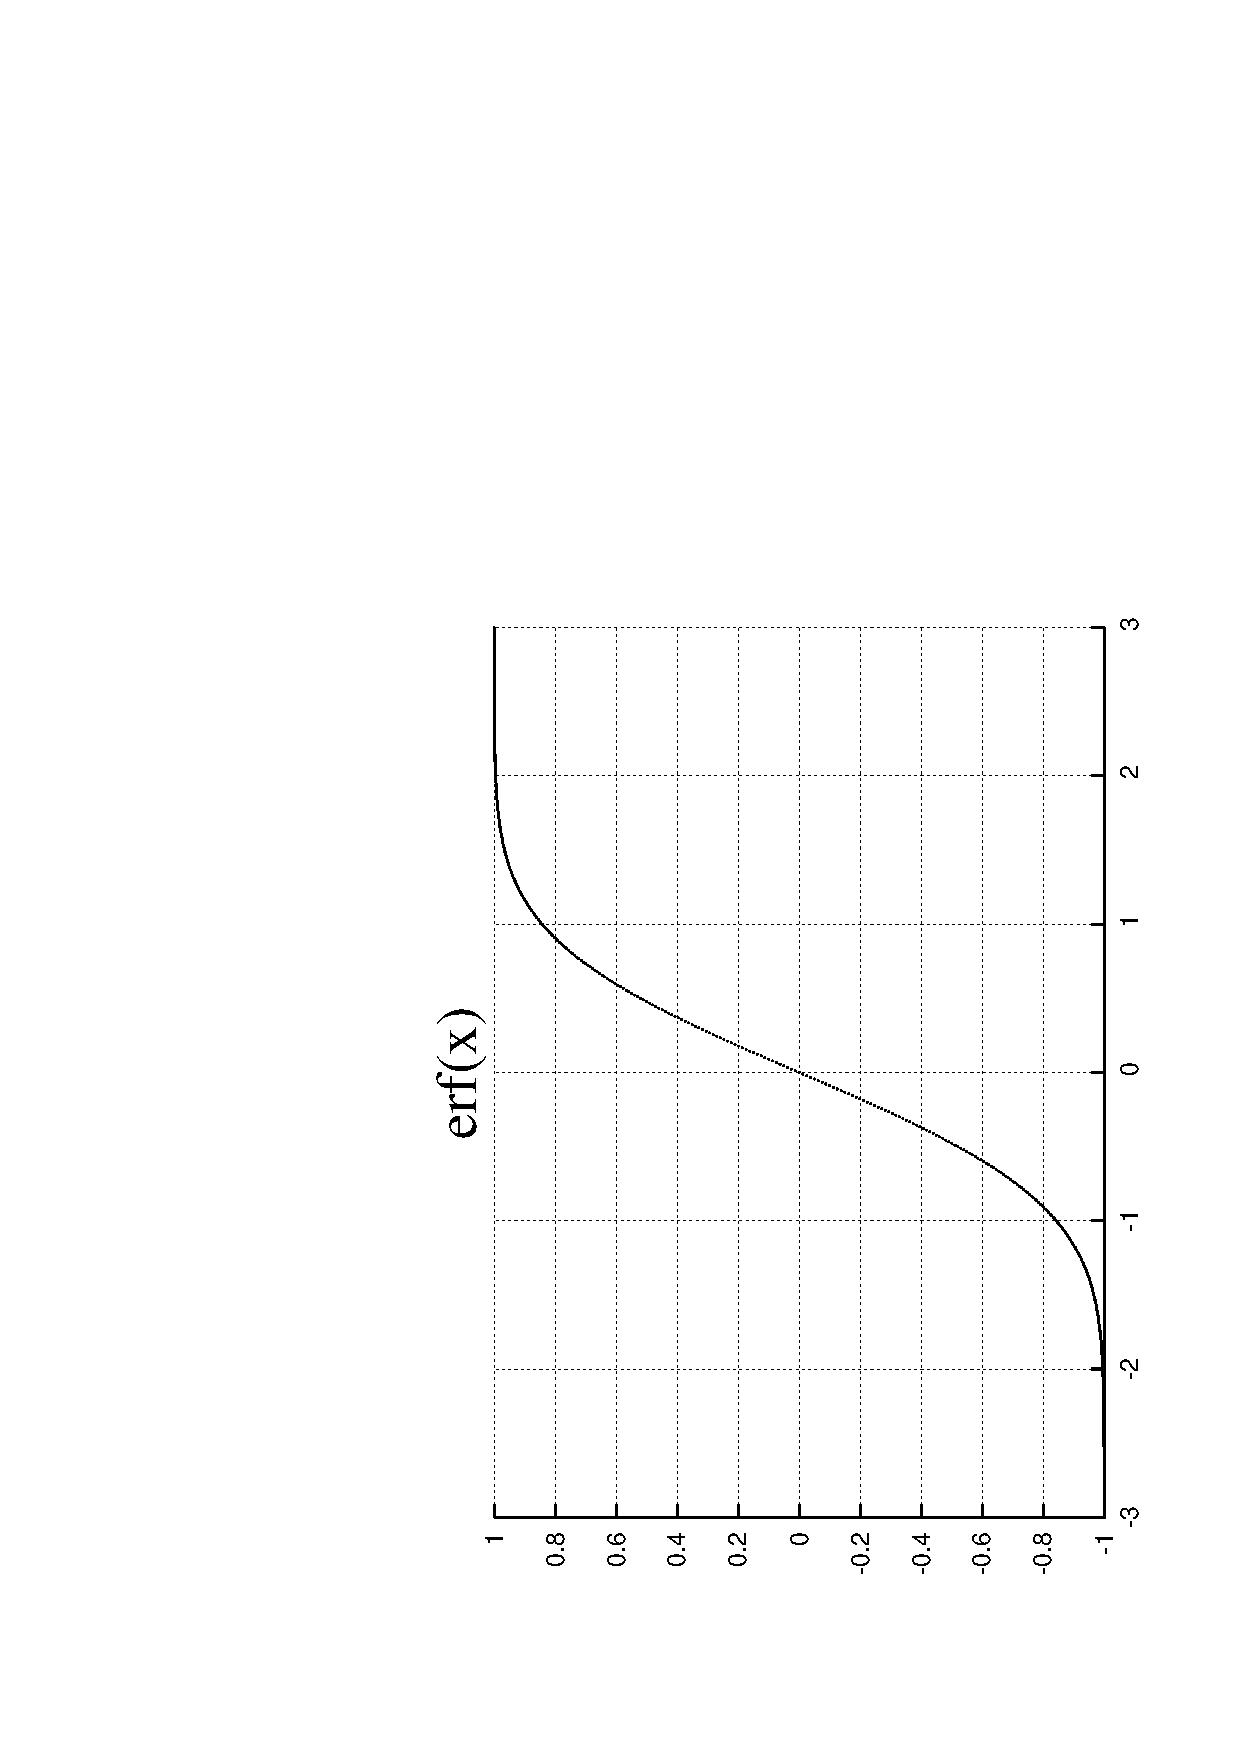
\includegraphics[bb=-90 0 400 250,width=1\textwidth] {chap2/erf}
\includegraphics[angle=-90,width=100mm]{chap2/erf.eps}
}
\end{center}
\caption{Error Function, from wiki}
\label{figure:errorfunction}
\end{figure*}

The implementation is a Java translation of c code from fdlibm53 written by Sun. There are a few ways to implement the error function, such as numerical integration, taylor expansion. But Sun's implementation is accurate and fast. The accuracy is 1ulp, the performance is ?ms per call on average.

\section{Complementary Error Function}
The complementary error function is defined as the following integral
\[ \operatorname{erfc}(x) = \frac{2}{\sqrt{\pi}} \int_x^{+\infty} e^{-t^2}dt\]
over the interval $(-\infty, \infty)$. $erfc(x)$ is the same integral as the error function, except the integral range now is over $(x, \infty)$ rather than $(0, x)$. It is easy to show 
\[ erf(x) + erfc(x) = 1\]
Here are more basic facts:
\begin{enumerate}
\item the range is between 0 and 2.
\item $erf(+\infty) = 0$ and $erf(-\infty) = 2$.
\item $erf(x)$ is strictly monotonely decreasing.
\end{enumerate}
The graph of the error function is below. 
\begin{figure*}[htp]
\begin{center}
{
\includegraphics[bb=-90 0 400 250,width=1\textwidth] {chap2/errorcfunction.png}
}
\end{center}
\caption{Complementary Error Function, from wiki}
\label{figure:errorcfunction}
\end{figure*}

One way to implement $erfc(x)$ is to use $1 - erf(x)$. However, when x is large and $erf(x)$ is near 1, this suffers from cancellation error. One way to fix this is to use BigDecimal when x is large.

Fortunately, Sun's fdlibm53 has an implmentation for the complementary error function too. The accuracy is 1ulp, the performance is ?ms. 


\section{Error Function Inverse}
Since the error function is strictly increasing on the entire real axis, the inverse function exists in $(-1, 1)$. The implementation is a translation of c code from cephes. performance? 



%********** End of chapter **********

\chapter{More Matrix Operations}
\minitoc
Now we are ready to consider these operations. We provide our own implementation and Jlapack hookup. There is no point to reinvent the wheel if there is a high quality package available. Better algorithms are added over time, such as divide-and-conquer, parallel. 

Template methods for iterative methods.

Estimate run time $O(n^3)$

\section{Matrix Norms}
There are many norms

\section{Matrix Decompositions}
We consider only the commonly used decompositions.

\subsection{LU Decomposition}
Pivoting: no partial or full.

Full LU decomposition is numerical stable for well conditioned matrices.

Lapack SGETRF

\subsection{Cholesky Decomposition}
If a matrix is symmetric, then the LU decomposition can be simplified
\[A = L * D * L^T\]
where L is an unit lower triangular matrix and D is diagonal. If A is positive definite, then we can absorb D into L by taking the square root of the cells of D, \[A= L * L^T\]
Numerically, Cholesky decomposition takes a shortcut using the above expression and thus save time. If A is not positive definite, in theory we still have the first expression, but due to pivoting we can't use it numerically. The best shot is to make D is block diagonal with 2 X 2 blocks.
\subsection{QR Decomposition}
Using householder transformation.

\subsection{Singular Value Decomposition(SVD)}
Do we care symmetric?

Polar decomposition of a matrix A is A = PQ, where P is symmetric positive semidefinite and Q is orthogonal. We can derive this from the SVD.

\subsection{Eigen Decomposition}
This part has several applications:
\begin{itemize}
\item find eigenvalues only
\item find eigenvalues and eigenvectors
\item find eigenvalues, eigenvectors, and the transformation matrix.
\end{itemize}
If the matrix is symmetric, we could use householder matrix to transform it to a tridiagonal matrix, then use QL + implicit shift.

If the matrix is nonsymmetric, use householder to transform it to a Hessenberg form, then transform it to a Schur form.

\section{Determinant}
We could use LU decomposition to compute Determinant for general matrices.

\section{Linear Equation Systems}
Use LU decomposition to solve. pivoting.

general solver()

--> LU

--> cholesky

--> Iterative

Another method is iterative method.
Here are the two packages:

SPARSKIT: http://www-users.cs.umn.edu/~saad/software/

Templates: http://www.netlib.org/templates/
\section{Matrix Inverse and Condition Number}
The inverse of a matrix can be deducted from the linear solver.
The condition number is defined as \[\kappa = {\frac{1}{|A||A^{-1}}|}\]
condition number estimate.

\section{Testing}
test different compositions.
\subsection{Correctness and Error Bound}
\subsection{Algorithm Stability}
\subsection{Performance}
In general, there are two places where we can optimize:

     *      1. time spent to access elements

     *      2. time spent to calculate.

Java array bound checking.

Test the difference between:

Matrix and double[][]

and 

Vector and double[]

for getter/setter.
\section{Reference}

Java implementations:
\begin{itemize}
\item JLapack: http://www.netlib.org/lapack/
\item Colt implementation:
\item Jsci implementation:
\item ojAlgo
\item Jama
\item Jampack
\item UJMP: http://www.ujmp.org/
\end{itemize}

Other implementations:
\begin{itemize}
\item Aglib: for C++, .net
\item newmat: a good C++ implementation
\item BLAS: http://www.netlib.org/blas/
\item BOOST: http://www.boost.org/ 
\item PLapack C implementation: http://www.cs.utexas.edu/~plapack/
\end{itemize}

BLAS

\begin{thebibliography}{99}

% >>>>>>>>> Book examples <<<<<<<<<
\bibitem{CarpenterBOOK} Carpenter, R.H.S., {\textit Movements of the Eyes},
 2nd Edition, Pion Publishing, 1988.

\bibitem{FranklinBOOK} Franklin, G.F., Powel, J.D., Workman, M.L.,
{\textit Digital Control of Dynamic Systems}, Second Edition,
Addison-Wesley, 1990.

% >>>>>>>>> Conference Proceedings Example <<<<<<<<<
\bibitem{OhICRA1998} Oh, P.Y., Allen, P.K., ``Design a Partitioned
 Visual Feedback Controller,'' {\textit IEEE Int Conf Robotics
 \& Automation}, Leuven, Belgium, pp. 1360-1365 5/98

% >>>>>>>>> Journal Example <<<<<<<<<<<<<<<<<<<<<<<<
\bibitem{OhTRA2001} Oh, P.Y., Allen, P.K., ``Visual Servoing
 by Partitioning Degrees of Freedom,'' {\textit IEEE Trans on 
 Robotics \& Automation}, V17, N1, pp. 1-17, 2/01

\end{thebibliography}

\chapter{Beta Function}
\minitoc
In this chapter, we discuss the Beta function related functions, namely, Beta Fucntion and incomplete Beta function.

\section{Beta Function}
The Beta function is definted in terms of the Gamma function:
\[ B(x, y) = \frac{\Gamma(x)\Gamma(y)}{\Gamma(x + y)} = \int_0^1 t^{x-1}(1-t)^{y-1}dt\]
for $x > 0$ and $y > 0$. Here are some basic facts about the beta function:
\begin{enumerate}
\item Beta function is symmetric, $B(x, y) = B(y, x)$.
\item For any real x in the domain, $\Gamma(x) = x\Gamma(x-1)$.
\item For any real x in the domain, 
\[\Gamma(1 - x)\Gamma(x) = \frac{\pi}{sin(\pi x)}\] 
This is called Euler's reflection and can be used to compute gamma function values for negative x if we know the values for positive x.
\end{enumerate} 
The graph for the beta function is below.
\begin{figure*}[htp]
\begin{center}
{
\includegraphics[bb=0 0 480 300,width=1\textwidth] {chap4/beta.png}
}
\end{center}
\caption{Incomplete Beta Function, from Boost}
\label{figure:betafunction}
\end{figure*}

\section{Incomplete Beta Function}
The incomplete Beta function is defined as
\[ B(x; a, b) = \int_0^x t^{a-1}(1-t)^{b-1}dt\]
for $a > 0$, $b > 0$, and $0 < x < 1$. The regularized incomplete Beta function is defined as
\[ I_x(a, b) = \frac{B(x; a, b)}{B(a, b)}\]
similar to the case of incomplete gamma function. Similarly, we could define the complementary regulaized incomplete beta function.
Here are some basica facts about the incomplete beta function:

The graph is below
\begin{figure*}[htp]
\begin{center}
{
\includegraphics[bb=0 0 480 300,width=1\textwidth] {chap4/inbeta.png}
}
\end{center}
\caption{Incomplete Beta Function, from Boost}
\label{figure:incompletebetafunction}
\end{figure*}

\begin{thebibliography}{99}

% >>>>>>>>> Book examples <<<<<<<<<
\bibitem{Demmel@1997} Demmel, J.W., {\itshape Applied Numerical Linear Algebra},
 SIAM, 1997.
\bibitem{GolubLoan} Golub, G.H., Loan, C.F., {\itshape Matrix Computations},
 3rd Edition, The Johns Hopkins University Press, 1996.


\end{thebibliography}


% *************** Bibliography ***************
%\bibliographystyle{plain}
%{\small\bibliography{Design_And_Implementation}}

\backmatter

\end{document}
